\paragraph{}Ta projektna naloga se osredotoča na strukturo in razvoj zadnje različice aplikacije 3.0. Ta je objavljena na spletni trgovini Google Play na naslovu \url{https://play.google.com/store/apps/details?id=com.zigapk.gimvic.suplence}. Aplikacija je odprtokodna, njena izvorna koda pa je dostopna na spletnem portalu Github na naslovu \url{https://github.com/GimVic-app/gimvic-android/}.

\subsection{Pridobivanje podatkov}
\paragraph{}Podatki, ki jih aplikacija potrebuje se nahajajo na več različnih strežnikih v zelo različnih oblikah. Podatki o nadomeščanjih se pridobijo s primerno zavarovane spletne storitve spletne redovalnice Gimnazije Vič v JSON\cite{json-wiki} (JavaScript Object Notation). Podatki o urniku za vse razrede in učitelje so na voljo na naslovu \url{http://old.gimvic.org/urnik/data.js} v obliki JavaScript izvorne kode, ki generira tabelo. Sistem za pridobivanje podatkov o jedilniku pa takrat še ni bil zastavljen.

\paragraph{}Jedilnik sestavlja ga. Eva Jelen na svojem računalniku v Excelu. Da bi podatke lahko spravili in obdelali na strežniku, sem pripravil vtičnik za Excel, dostopen na \url{https://github.com/GimVic-app/menu-uploader}. Tega sem namestil na njen računalnik, tako da lahko z enim samim klikom posodobi podatke o jedilniku.

\paragraph{}Da se izognemo brezpotrebnemu in zahtevnemu obdelovanju podatkov na telefonu, se vsi podatki zberejo na strežnikiu in obdelajo ter shranijo v relacijsko podatkovno bazo MySQL\cite{mysql-wiki}. Aplikacija lahko tako s preprosto poizvedbo na strežnik dobi vse podatke v JSON\cite{json-wiki} obliki. Uporabnikove nastavitve aplikacija definira kar z URL parametri\cite{query-wiki}. Podatki, ki jih strežnik vrne, vsebujejo seznam dni in za vsak dan natančno opisan urnik, morebitna nadomeščanja ter jedilnik.

\subsection{Struktura aplikacije}
\paragraph{}Aplikacija je sestavljena iz večih aktivnosti. Med njimi najpomembnejše so:
\begin{itemize}
  \setlength\itemsep{0em}
  \item upravilej podatkov,
  \item glavna aktivnost,
  \item nastavitve,
  \item aktivnost za izbiranje filtrov.
\end{itemize}

\subsubsection{Upravitelj podatkov}
\paragraph{}Upravitelj podatkov podaja informacije glavni aktivnosti. Te pridobiva v rednih intervalih s strežnika. V poizvedbah strežniku poda tudi uporabnikove nastavitve. Če glavna aktivnost potrebuje podatke, internetne povezave pa ni, upravitelj podatkov poda zadnje podatke, ki so shranjeni na napravi skupaj z datumom in časom zadnje posodobitve.

\subsubsection{Glavna aktivnost}
\paragraph{}Glavna aktivnost (slika \ref{fig:main_activity}) uporabniku prikazuje podatke o njegovem urniku ter jedilniku. Omogoča preprosto pomikanje med posameznimi dnevi ter vsebuje tudi gumb za dostop do nastavitev. Podatke za prikazovanje dobi iz upravitelja podatkov.

\subsubsection{Nastavitve}
\paragraph{}Nastavitve (slika \ref{fig:settings_activity}) omogočajo uporabniku nastavljanje vrste malice in prikazovanja nadomeščanj. Vsebujejo tudi gumb, ki uporabnika popelje na stran za izbiro razredov ter osnovne podatke o različici in avtorju aplikacije.

\subsubsection{Izbira filtrov}
\paragraph{}Aktivnost za izbiro filtrov (slika \ref{fig:filters_activity}) dijakom omogoča, da izberejo svoj razred in morebitne izbirne predmete, profesorjem pa da izberejo svoj urnik. Po dogovoru z ravnateljico mag. Alenko Krapež je izbira razreda omejena na 5 sprememb, izbira profesorja pa zaščitena z univerzalnim profesorskim geslom.

% images
\begin{figure}[!htb]
\minipage{0.32\textwidth}
  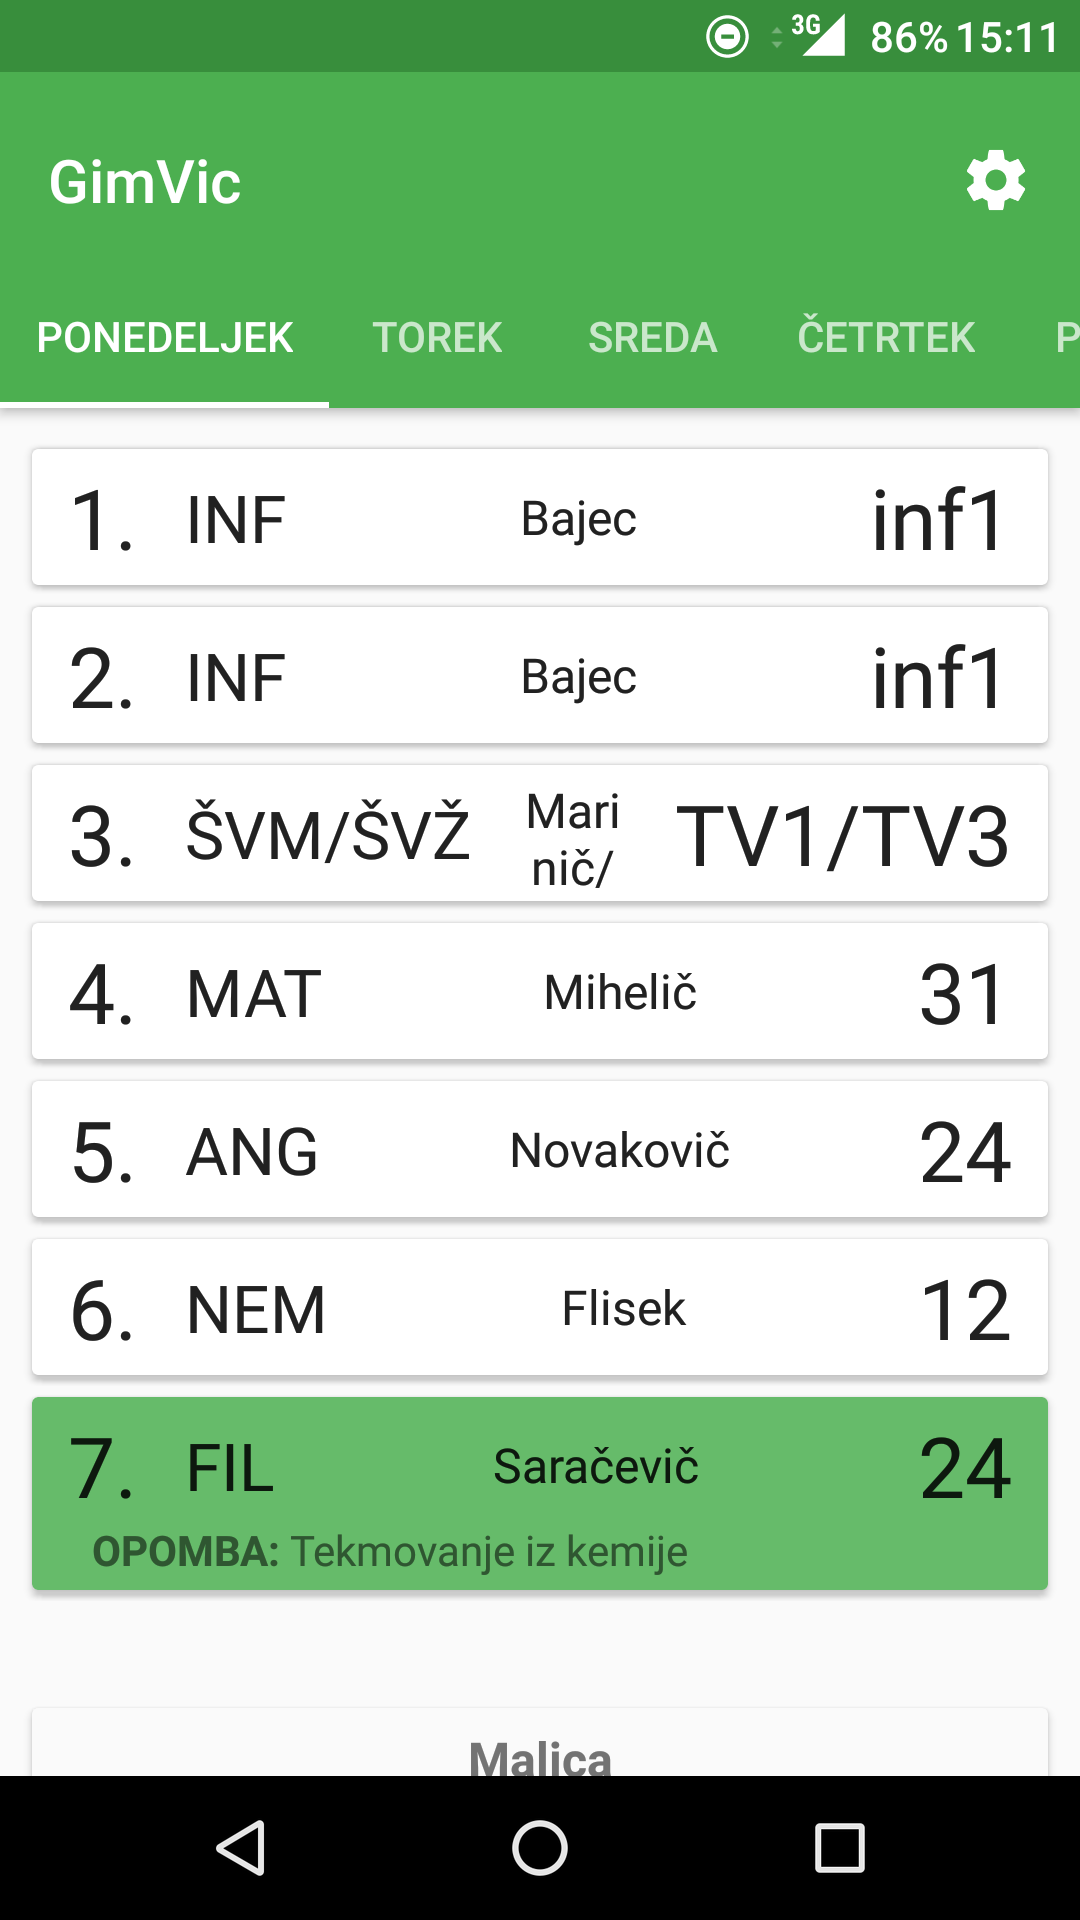
\includegraphics[width=\linewidth]{images/main.png}
  \caption{Glavna stran}\label{fig:main_activity}
\endminipage\hfill
\minipage{0.32\textwidth}
  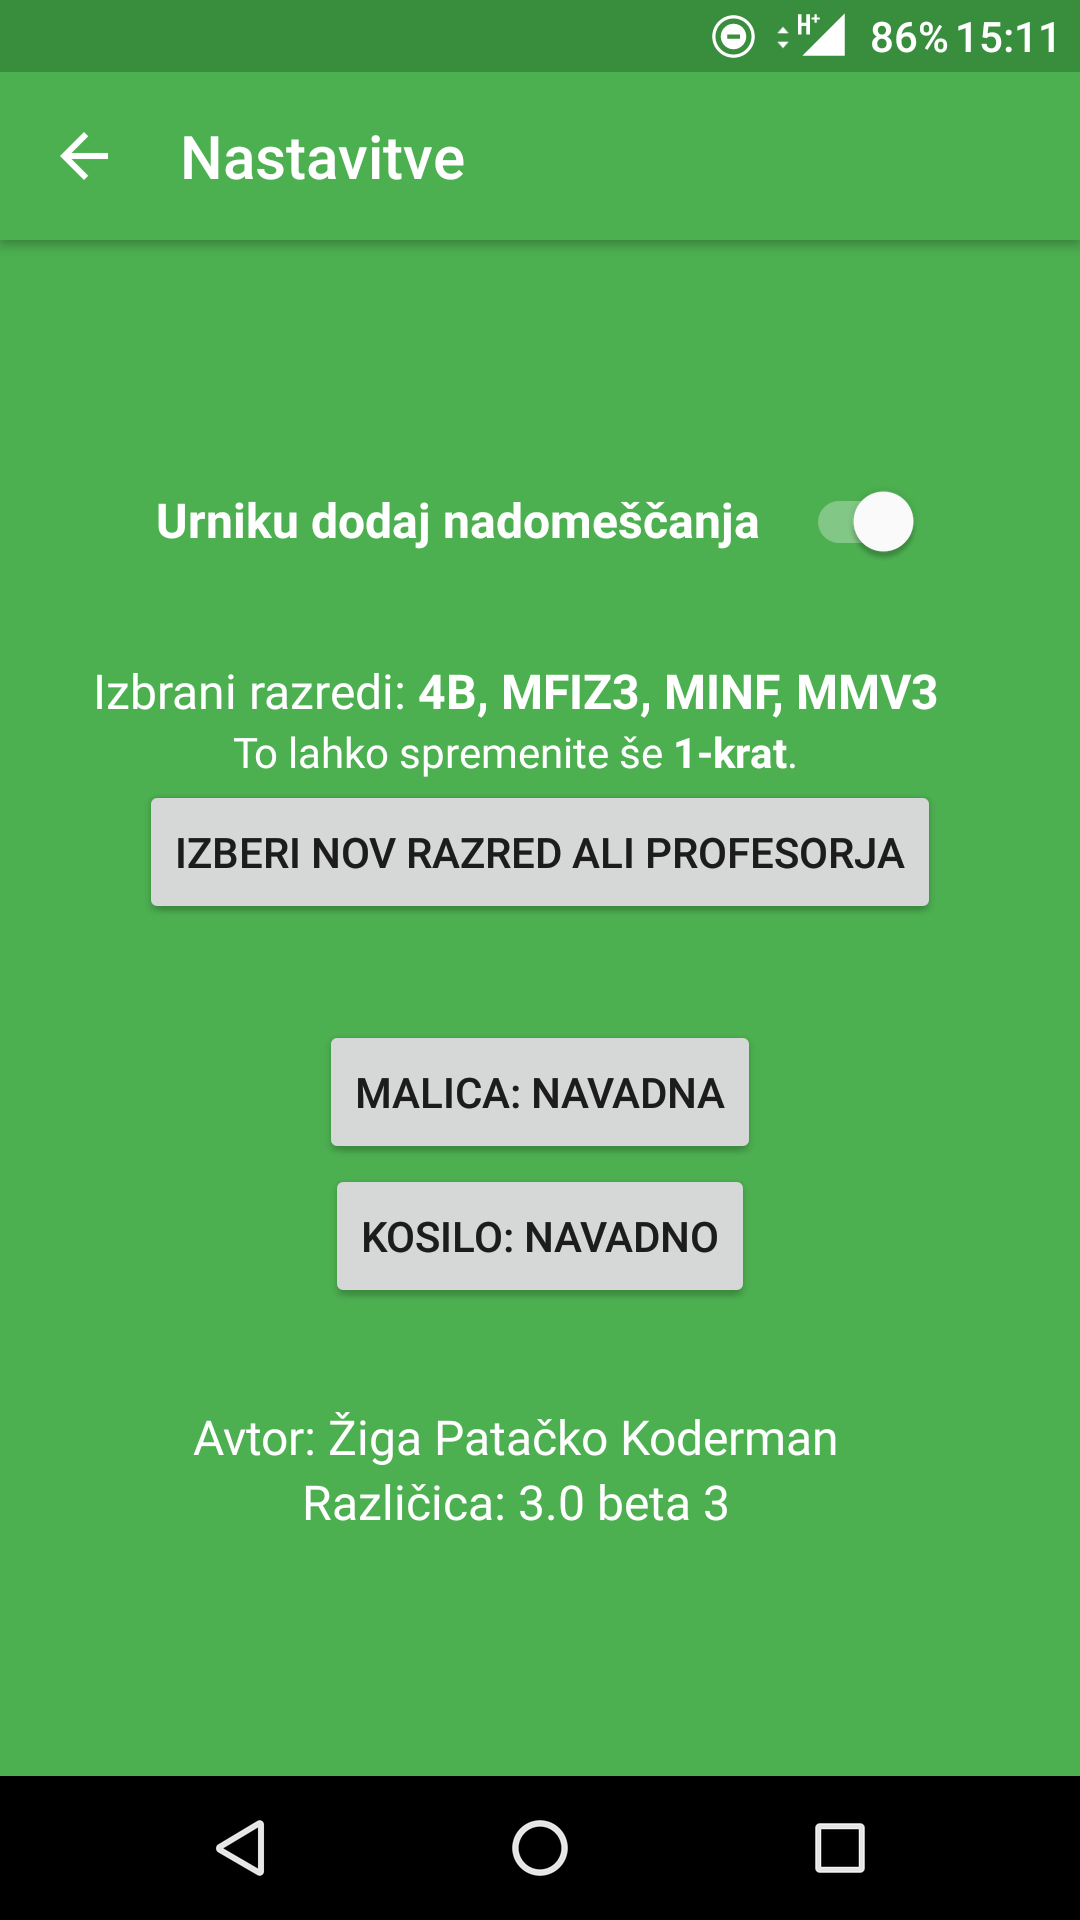
\includegraphics[width=\linewidth]{images/settings.png}
  \caption{Nastavitve}\label{fig:settings_activity}
\endminipage\hfill
\minipage{0.32\textwidth}%
  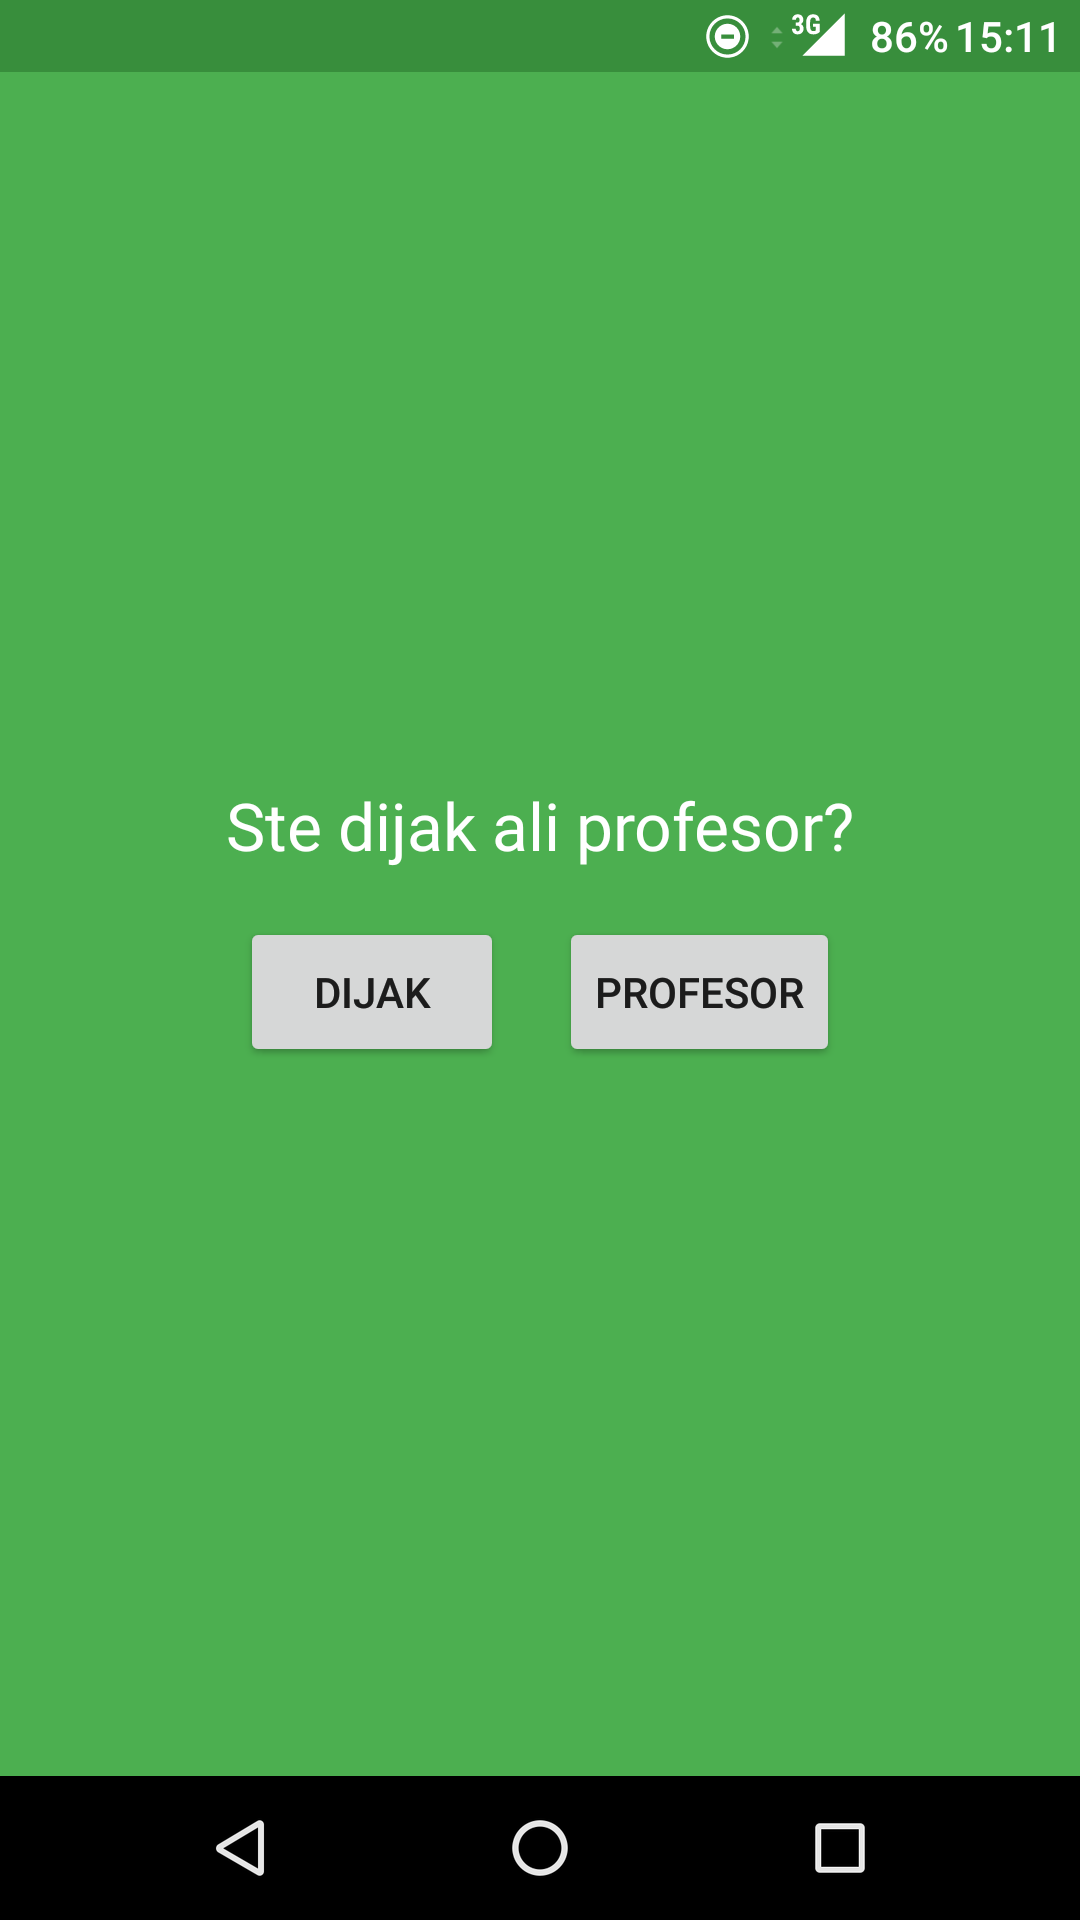
\includegraphics[width=\linewidth]{images/filters.png}
  \caption{Izbira filtrov}\label{fig:filters_activity}
\endminipage
\end{figure}
